%%%%%%%%%%%%%%%%%%%%%%%%%%%%%%%%%%%%%%%%%
% Beamer Presentation
% LaTeX Template
% Version 1.0 (10/11/12)
%
% This template has been downloaded from:
% http://www.LaTeXTemplates.com
%
% License:
% CC BY-NC-SA 3.0 (http://creativecommons.org/licenses/by-nc-sa/3.0/)
%
%%%%%%%%%%%%%%%%%%%%%%%%%%%%%%%%%%%%%%%%%

%----------------------------------------------------------------------------------------
%	PACKAGES AND THEMES
%----------------------------------------------------------------------------------------

\documentclass{beamer}

\mode<presentation> {

% The Beamer class comes with a number of default slide themes
% which change the colors and layouts of slides. Below this is a list
% of all the themes, uncomment each in turn to see what they look like.

%\usetheme{default}
%\usetheme{AnnArbor}
%\usetheme{Antibes}
%\usetheme{Bergen}
%\usetheme{Berkeley}
%\usetheme{Berlin}
%\usetheme{Boadilla}
%\usetheme{CambridgeUS}
%\usetheme{Copenhagen}
%\usetheme{Darmstadt}
%\usetheme{Dresden}
%\usetheme{Frankfurt}
%\usetheme{Goettingen}
%\usetheme{Hannover}
%\usetheme{Ilmenau}
%\usetheme{JuanLesPins}
%\usetheme{Luebeck}
\usetheme{Madrid}
%\usetheme{Malmoe}
%\usetheme{Marburg}
%\usetheme{Montpellier}
%\usetheme{PaloAlto}
%\usetheme{Pittsburgh}
%\usetheme{Rochester}
%\usetheme{Singapore}
%\usetheme{Szeged}
%\usetheme{Warsaw}

% As well as themes, the Beamer class has a number of color themes
% for any slide theme. Uncomment each of these in turn to see how it
% changes the colors of your current slide theme.

%\usecolortheme{albatross}
%\usecolortheme{beaver}
%\usecolortheme{beetle}
%\usecolortheme{crane}
%\usecolortheme{dolphin}
%\usecolortheme{dove}
%\usecolortheme{fly}
%\usecolortheme{lily}
%\usecolortheme{orchid}
%\usecolortheme{rose}
%\usecolortheme{seagull}
%\usecolortheme{seahorse}
%\usecolortheme{whale}
%\usecolortheme{wolverine}

%\setbeamertemplate{footline} % To remove the footer line in all slides uncomment this line
%\setbeamertemplate{footline}[page number] % To replace the footer line in all slides with a simple slide count uncomment this line

%\setbeamertemplate{navigation symbols}{} % To remove the navigation symbols from the bottom of all slides uncomment this line
}

\usepackage{amsmath}
\usepackage{outlines}
\usepackage{fancyvrb}
\usepackage{listings}
\usepackage{graphicx} % Allows including images
\usepackage{booktabs} % Allows the use of \toprule, \midrule and \bottomrule in tables
\usepackage{tikz}
%%%<
\usepackage{verbatim}
% \usepackage[active,tightpage]{preview}
\usetikzlibrary{shadows}
\usetikzlibrary{shapes.multipart}
\usetikzlibrary{positioning}
% \PreviewEnvironment{tikzpicture}
% \setlength\PreviewBorder{5pt}%
%%%>

%----------------------------------------------------------------------------------------
%	TITLE PAGE
%----------------------------------------------------------------------------------------

\title[]{Introduction to Nodal Method For Reactor Analysis} % The short title appears at the bottom of every slide, the full title is only on the title page

\author{Muhammad Imron} % Your name

\begin{document}

\begin{frame}
\titlepage % Print the title page as the first slide
\end{frame}

\begin{frame}
\frametitle{Overview} % Table of contents slide, comment this block out to remove it
\tableofcontents % Throughout your presentation, if you choose to use \section{} and \subsection{} commands, these will automatically be printed on this slide as an overview of your presentation
\end{frame}

%----------------------------------------------------------------------------------------
%	PRESENTATION SLIDES
%----------------------------------------------------------------------------------------

%------------------------------------------------
\section{Introduction} % Sections can be created in order to organize your presentation into discrete blocks, all sections and subsections are automatically printed in the table of contents as an overview of the talk
%------------------------------------------------


\begin{frame}
\frametitle{Introduction}
\begin{itemize}
\item Since it was proposed more than 40 years ago, nodal method has become a standard tool for many modern reactor simulators to perform routine reactor core calculations and safety analysis for commercial nuclear power plants.
\item Nodal method reduces the number of unknowns by factor of hundreds or even thousands that allows reactor simulators to solve reactor problems rapidly compared to traditional Finite Difference Method (FDM).
\item It also enables reactor spatial-kinetic calculations, instead of point kinetic, to be accomplished in today’s computers with acceptable running time.
\end{itemize}
\end{frame}

%------------------------------------------------

\begin{frame}
\frametitle{Introduction}
\begin{columns}[c] % The "c" option specifies centered vertical alignment while the "t" option is used for top vertical alignment

\column{.65\textwidth} % Left column and width
\textbf{Typical PWR Core}
\begin{figure}
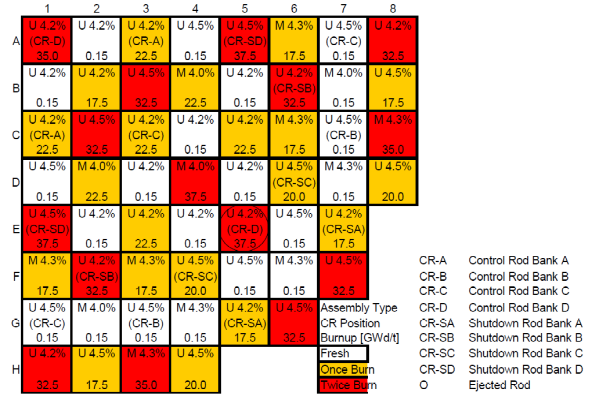
\includegraphics[width=0.8\linewidth]{core.png}
\end{figure}
\vspace{2cm}
Images from [1]

\column{.35\textwidth} % Right column and width
\begin{figure}
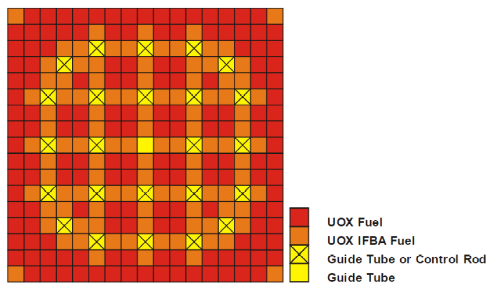
\includegraphics[width=0.8\linewidth]{FA.png}
\end{figure}
\begin{block}{Number of nodes for FDM}
\footnotesize{17x17x45x180x2 = 4,681,800}
\end{block}
\begin{block}{Number of nodes for Nodal Method}
\footnotesize{2x2x45x36x2 = 12,960}
\end{block}


\end{columns}
\end{frame}

%------------------------------------------------

\begin{frame}
\frametitle{Introduction}
\begin{table}{}
  \caption{IAEA2D Problem}
  \begin{tabular}{p{2cm}p{3cm}p{2.5cm}p{2cm}}
  \toprule
  \textbf{Code Methods} & \textbf{Number of mesh or nodes} & \textbf{Running Time (second)} & \textbf{\emph{K-eff}}\\
  \midrule
  FDM & 10,816 & 6.7 & 1.029541  \\
  Nodal & 169 & 0.02 & 1.029600  \\
  \bottomrule
  \end{tabular}
  \medskip
  \raggedright{Error on effective multiplication factor is 5.9 pcm}
\end{table}

\begin{table}{}
\caption{IAEA3D Problem}
\begin{tabular}{p{2cm}p{3cm}p{2.5cm}p{2cm}}
  \toprule
  \textbf{Code Methods} & \textbf{Number of mesh or nodes} & \textbf{Running Time (second)} & \textbf{\emph{K-eff}}\\
  \midrule
  FDM & 2,055,040 & 1094 & 1.029013 \\
  Nodal & 3,211 & 0.2 & 1.029082  \\
  \bottomrule
  \end{tabular}
  \medskip
  \raggedright{Error on effective multiplication factor is 6.9 pcm}
\end{table}

\end{frame}

%------------------------------------------------

\begin{frame}{Introduction}
  \begin{figure}{IAEA3D Axially Averaged Power Distribution}
  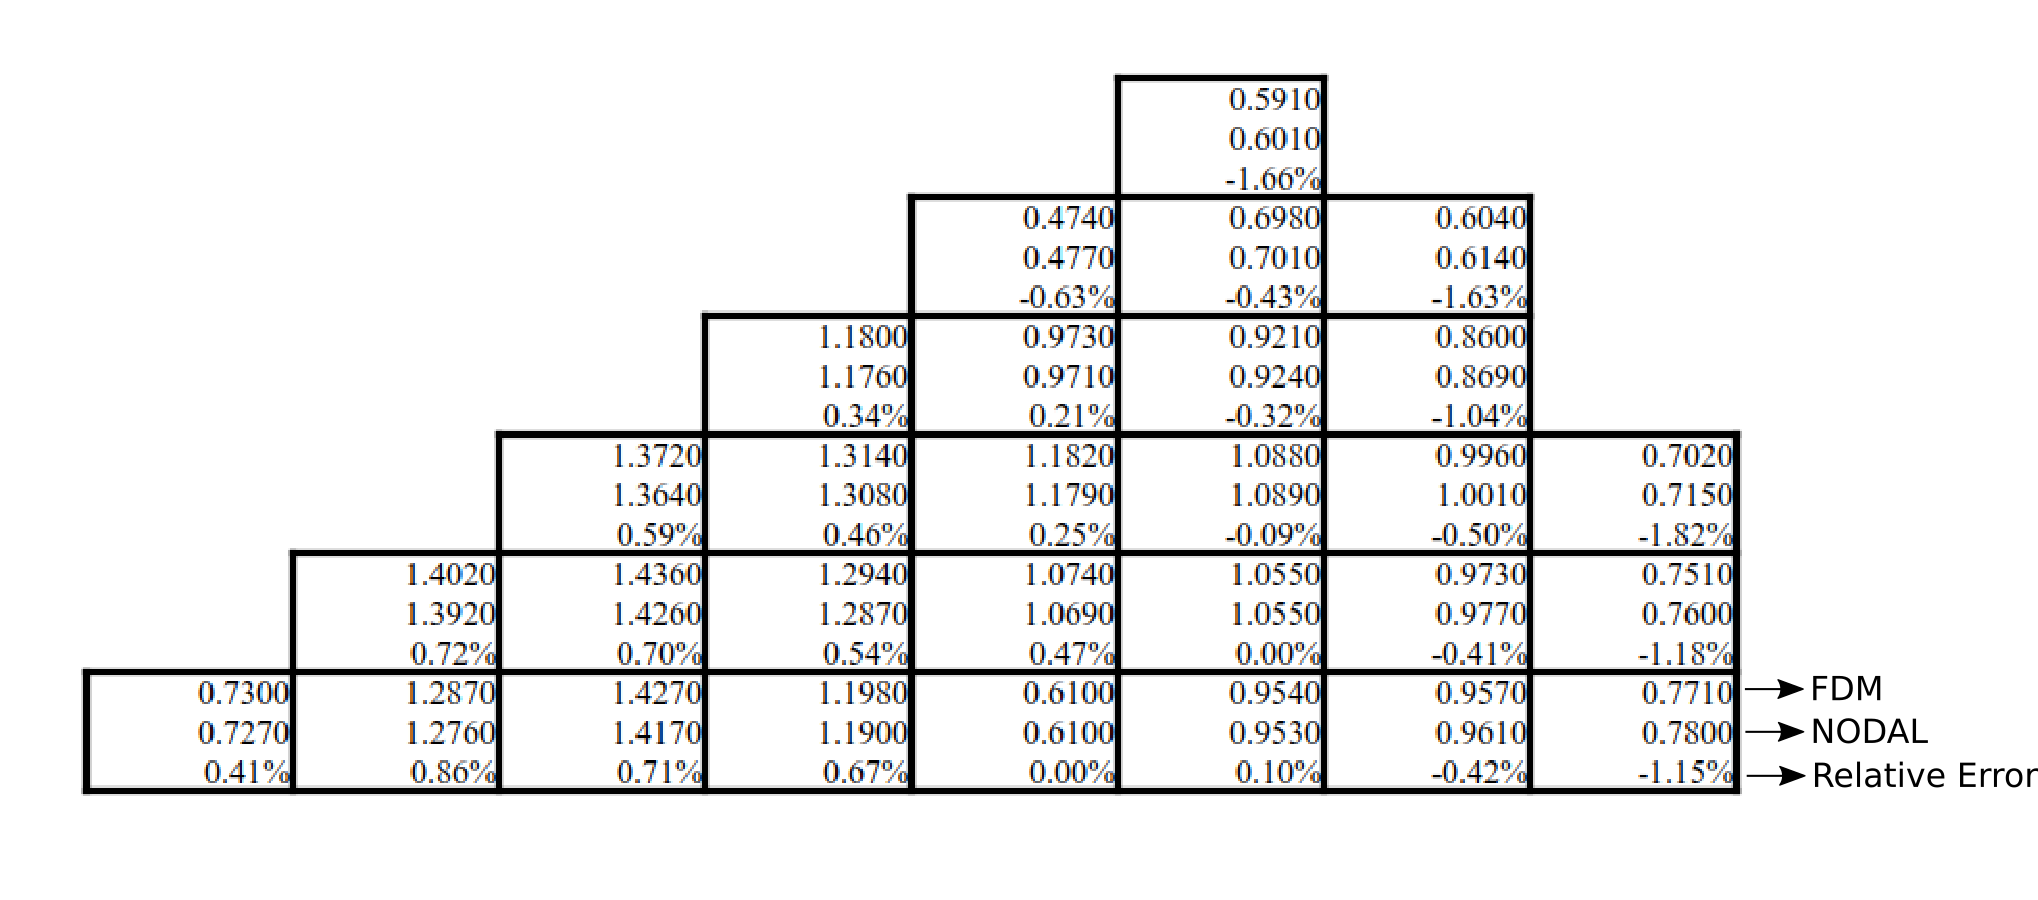
\includegraphics[width=1.0\linewidth]{power.png}
  \end{figure}
\end{frame}

%------------------------------------------------

\begin{frame}
\frametitle{Introduction}
\begin{table}{}
  \caption{UO2-MOX PWR 3D Transient Problem}
  \begin{tabular}{p{3.0cm}p{1.5cm}p{2cm}p{2cm}p{1.5cm}}
  \toprule
  \textbf{Codes} & \textbf{Peak time (s)} & \textbf{Peak Power (\%)} & \textbf{Reactivity Peak (\$)} & \textbf{Integral Power (\%.s)}\\
  \midrule
  Serpent-SCF [2] & 0.35 & 179$\pm$26 & 1.18$\pm$0.02 & 27.7  \\
  ADPRES $2G$ & 0.35 & 173 & 1.12 & 30.4  \\
  PARCS $2G$ [1] & 0.34 & 142 & 1.12 & 27.2  \\
  PARCS $4G$ [1] & 0.33 & 152 & 1.12 & 27.8  \\
  PARCS $8G$ [1] & 0.32 & 172 & 1.14 & 29.1  \\
  \bottomrule
  \end{tabular}
  \begin{flushleft}
    \textbf{CPU Time (mins)} \\
    \textbf{Serpent-SCF}: 9,600,00 (about 18 years). The simulation was done on a cluster with 1280 processors (@2.6GHz) and it took about 120 hours  \\
    \textbf{ADPRES}: 5
  \end{flushleft}
\end{table}
\end{frame}

%------------------------------------------------
\section{Nodal Method}
%------------------------------------------------

\begin{frame}[fragile]{Nodal Method Implementation}
  \tikzstyle{abstract}=[rectangle, draw=black, rounded corners, fill=blue!40, drop shadow,
          text centered, anchor=north, text=white, text width=3cm]
  \tikzstyle{comment}=[rectangle, draw=black, rounded corners, fill=green, drop shadow,
          text centered, anchor=north, text=white, text width=3cm]
  \tikzstyle{line}=[-, thick]
  \begin{figure}
  \begin{tikzpicture}[node distance=2.3cm]
      \node (Item) [abstract]
          {
              \textbf{Nodal Method Implementation}
          };
      \node (AuxNode01) [text width=0.6cm, below=of Item] {};
      \node (Component) [abstract, rectangle split, rectangle split parts=2, left=of AuxNode01]
          {
              \textbf{CMFD \linebreak Formulation} [6]
              \nodepart{second}PARCS [7], NESTLE [8], NODAL3 [9], ADPRES, etc
          };
      \node (System) [abstract, rectangle split, rectangle split parts=2, right=of AuxNode01]
          {
              \textbf{Response Matrix Formulation} [3], [4], [5]
              \nodepart{second}MOSRA-Light [5] and older nodal computer codes
          };

      \draw[line] (Component.north) -- ++(0,0.8) -| (Item.south);
      \draw[line] (Component.north) -- ++(0,0.8) -| (System.north);


  \end{tikzpicture}
\end{figure}
\end{frame}

%------------------------------------------------

\begin{frame}
\frametitle{Coarse Mesh Finite Difference}
\begin{block}{The Neutron Diffusion Equation}
    \begin{equation}
      \begin{split}
      \frac{\partial }{{\partial x}}J_{gx}(x,y,z) + \frac{\partial }{{\partial y}}J_{gy}(x,y,z) + \frac{\partial }{{\partial z}}J_{gz}(x,y,z) + \Sigma _{r,g}(x,y,z)\phi _g(x,y,z) \\
       = \frac{{\chi _g}}{{{k_{eff}}}}\sum\limits_{g' = 1}^G {\nu \Sigma _{f,g'}(x,y,z)\phi _{g'}(x,y,z)} + \sum_{\substack{g'=1 \\ g'\neq g}}^G {\Sigma _{s,g' \to g}(x,y,z)\phi _{g'}(x,y,z)}  \label{ndif}
     \end{split}
    \end{equation}
\end{block}
\begin{block}{Fick's Law}
  \begin{equation}
  J_{gx}(x,y,z) =  - D_g(x,y,z)\frac{\partial }{{\partial x}}\phi _g^k(x,y,z)  \label{eq:fick}
  \end{equation}
\end{block}
\end{frame}

%------------------------------------------------

\begin{frame}
\frametitle{Coarse Mesh Finite Difference}
\begin{block}{Integrating over node $k$ which is defined as}
    \begin{equation}
      { \scriptscriptstyle \left( { - \frac{1}{2}\Delta _x^k \le x \le \frac{1}{2}\Delta _x^k} \right),
      \left( { - \frac{1}{2}\Delta _y^k \le y \le \frac{1}{2}\Delta _y^k} \right),
      \left( { - \frac{1}{2}\Delta _z^k \le z \le \frac{1}{2}\Delta _z^k} \right)}
    \end{equation}
\end{block}
\begin{block}{We obtain discretized form of the neutron diffusion equation}
    \begin{equation}
      { \scriptscriptstyle \frac{1}{{\Delta _x^k}}\left( {J_{gx + }^k - J_{gx - }^k} \right) + \frac{1}{{\Delta _y^k}}\left( {J_{gy + }^k - J_{gy - }^k} \right) + \frac{1}{{\Delta _z^k}}\left( {J_{gz + }^k - J_{gz - }^k} \right) + \Sigma _{r,g}^k\overline \phi  _{g}^k = \overline Q _{g}^k} \label{eq:dif}
    \end{equation}
\end{block}
\begin{figure}
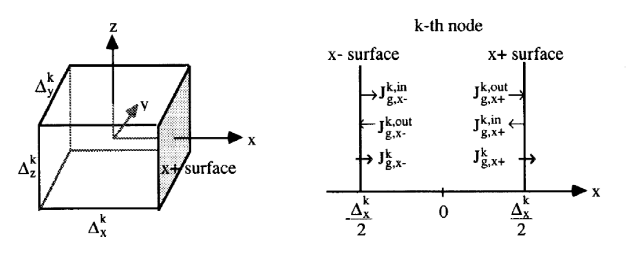
\includegraphics[width=0.6\linewidth]{int.png}
\end{figure}
\begin{flushleft}
  Image from [5]
\end {flushleft}
\end{frame}

%------------------------------------------------

\begin{frame}
\frametitle{Coarse Mesh Finite Difference}
\begin{block}{Where in Eq. \eqref{eq:dif}}
    \begin{equation}
      \begin{split}
      \overline \phi  _{g}^k = \frac{1}{{{V_k}}}\int_{ - \Delta x/2}^{ + \Delta x/2} {dx} \int_{ - \Delta y/2}^{ + \Delta y/2} {dy} \int_{ - \Delta z/2}^{ + \Delta z/2} {dz{^{}}} \phi _g^k(x,y,z) \\
      \overline Q _{g}^k = \frac{1}{{{V_k}}}\int_{ - \Delta x/2}^{ + \Delta x/2} {dx} \int_{ - \Delta y/2}^{ + \Delta y/2} {dy} \int_{ - \Delta z/2}^{ + \Delta z/2} {dz{^{}}} Q_g^k(x,y,z) \\
      J_{gx \pm }^k = \frac{1}{{\Delta _y^k\Delta _z^k}}\int_{ - \Delta y/2}^{ + \Delta y/2} {dy} \int_{ - \Delta z/2}^{ + \Delta z/2} {dz{^{}}} J_{gx}^k\left( {x = \frac{{ \pm \Delta _x^k}}{2},y,z} \right) \nonumber
     \end{split}
   \end{equation}
   \begin{equation}
   {V^k} = \Delta _x^k\Delta _y^k\Delta _z^k \nonumber
   \end{equation}
\end{block}

\end{frame}

%------------------------------------------------

\begin{frame}
\frametitle{Coarse Mesh Finite Difference}
\begin{block}{Traditional Finite Difference Method (FDM)}
    \begin{equation}
      \begin{split}
      J_{gx \pm }^k = \mp \widetilde{D}_{gx \pm }^k \left( \phi  _{g}^{k\pm1} - \phi  _{g}^k \right)
      \end{split}
    \end{equation}
\end{block}
\begin{block}{Coarse Mesh Finite Difference (CMFD)}
    \begin{equation}
      \begin{split}
      J_{gx \pm }^k = \mp \widetilde{D}_{gx \pm }^k \left( \phi  _{g}^{k\pm1} - \phi  _{g}^k \right) - \widehat{D}_{gx \pm }^k \left( \phi  _{g}^{k\pm1} - \phi  _{g}^k \right) \label{eq:upd}
      \end{split}
    \end{equation}
\end{block}
\begin{equation}
  \widetilde{D}_{gx \pm }^k = \frac{2 D_{gx}^{k\pm1} D_{gx}^{k}}{D_{gx}^{k\pm1}\Delta _x^k + D_{gx}^{k}\Delta _x^{k\pm1}}
\end{equation}
\end{frame}

%------------------------------------------------

\begin{frame}
\frametitle{Nodal Update}
\begin{block}{Transverse integrated diffusion equation can be obtained, for example, by integrating Eq. \eqref{ndif} over $y$ and $z$}
    \begin{equation}
      \begin{split}
      \frac{d}{{dx}}\overline J _{gx}^k(x) + \Sigma _{r,g}^k\overline \phi  _{gx}^k(x) = \overline Q _{gx}^k(x) - \frac{1}{{\Delta _y^k}}L_{gy}^k(x) - \frac{1}{{\Delta _z^k}}L_{gz}^k(x) \label{eq:transv}
      \end{split}
    \end{equation}
\end{block}
\begin{block}{where}
    \begin{equation}
      \begin{split}
      \scriptscriptstyle \overline J _{gx}^k(x) = \frac{1}{{\Delta _y^k\Delta _z^k}}\int_{ - \Delta y/2}^{ + \Delta y/2} {dy} \int_{ - \Delta z/2}^{ + \Delta z/2} {dz{^{}}} J_{gx}^k\left( {x,y,z} \right) \\
      \scriptscriptstyle \overline \phi  _{gx}^k(x) = \frac{1}{{\Delta _y^k\Delta _z^k}}\int_{ - \Delta y/2}^{ + \Delta y/2} {dy} \int_{ - \Delta z/2}^{ + \Delta z/2} {dz{^{}}} \phi _g^k\left( {x,y,z} \right) \\
      \scriptscriptstyle L_{gy}^k(x) = \left. {\frac{1}{{\Delta _z^k}}\int_{ - \Delta z/2}^{ + \Delta z/2} {dz{^{}}} J_{gy}^k\left( {x,y,z} \right)} \right|_{y =  - \frac{{\Delta y}}{2}}^{y = \frac{{\Delta y}}{2}} \\
      \scriptscriptstyle L_{gz}^k(x) = \left. {\frac{1}{{\Delta _y^k}}\int_{ - \Delta y/2}^{ + \Delta y/2} {dy{^{}}} J_{gz}^k\left( {x,y,z} \right)} \right|_{z =  - \frac{{\Delta z}}{2}}^{z = \frac{{\Delta z}}{2}} \\
      \end{split}
    \end{equation}
\end{block}
\end{frame}

%------------------------------------------------

\begin{frame}
\frametitle{Nodal Update}
\begin{block}{The one-dimensional flux is approximated by}
    \begin{equation}
      \begin{split}
        \overline \phi  _{gx}^k(x) \cong \overline \phi  _{g,0}^k{f_0}(x) + \sum\limits_{n = 1}^4 {a_{gxn}^k} {f_n}(x), \text{in which} \left( { - \frac{{{\Delta _x}}}{2} \le x \le \frac{{{\Delta _x}}}{2}} \right)  \label{eq:exp}
      \end{split}
    \end{equation}
\end{block}
\begin{block}{The basis functions shall satisfy}
    \begin{equation}
      \frac{1}{\Delta _x} \int_{ - \Delta x/2}^{ + \Delta x/2} {dx} {f_n}(x) =
      \begin{cases}
      1,& \text{if } n = 0 \\
      0,& \text{otherwise}
      \end{cases}
    \end{equation}
\end{block}

\begin{itemize}
\item In Analytic Nodal Method (ANM), however, instead of approximating one-dimensional flux by polnomials, Eq. \eqref{eq:transv} is analytically solved
\item This is possible because Eq. \eqref{eq:transv} material within the node is homogeneous
\item However, this puts limit on ANM to solve reactor problems only with two-group energy
\end{itemize}

\textbf{}
\end{frame}

%------------------------------------------------

\begin{frame}{Nodal Method}
  \begin{itemize}
  \item Substituting Eq. \eqref{eq:exp} to one-dimensional form of Eq. \eqref{eq:fick}, one would obtain nodal solutions (not FDM solutions) for net currents (i.e $J_{gx \pm }^k$, $J_{gy \pm }^k$, and $J_{gz \pm }^k$)
  \item Using these corrected nodal net currents, now $\widehat{D}_{gx \pm }^k$, $\widehat{D}_{gx \pm }^k$, and $\widehat{D}_{gx \pm }^k$ in Eq. \eqref{eq:upd} can be updated
  \item To do so, we must determine nodal expansion coefficients $a_{gxn}^k$, $a_{gyn}^k$ and $a_{gzn}^k$ for $n=1,2,3,4$. This can be done by solving \textbf{Two Nodes Problem}, hence we need to determine $8G$ nodal expansion coefficients for both nodes (4 nodal expansion coefficients for each node and each group).
  \item Therefore, we need $8G$ equations to obtain the $8G$ nodal expansion coefficients.
  \item This process involves non-linear iteration
  \end{itemize}
\end{frame}

%------------------------------------------------

\begin{frame}{Nodal Method}
  \begin{outline}
  \1 These $8G$ equations are
    \2 $2G$ neutron balance equations $\rightarrow$ substituting Eq. \eqref{eq:exp} to the first term on LHS of the Eq. \eqref{eq:transv}, and integrating over $x$
    \2 $2G$ first moment equations $\rightarrow$ substituting Eq. \eqref{eq:exp} to Eq. \eqref{eq:transv}, weighting by $f_1(x)$, and integrating over $x$
    \2 $2G$ second moment equations $\rightarrow$ substituting Eq. \eqref{eq:exp} to Eq. \eqref{eq:transv}, weighting by $f_2(x)$, and integrating over $x$
    \2 $G$ flux continuity equations $\rightarrow$ solve Eq. \eqref{eq:exp} for $x = -\frac{\Delta _x^k}{2}$ and $x = \frac{\Delta _x^k}{2}$
    \2 $G$ net current continuity equations $\rightarrow$ substituting Eq. \eqref{eq:exp} to Eq. \eqref{eq:fick} and solve for $x = -\frac{\Delta _x^k}{2}$ and $x = \frac{\Delta _x^k}{2}$
  \1 These proceedures are also carried out for $y$ and $z$ directions
  \end{outline}
  \begin{figure}
  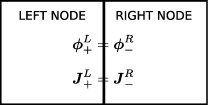
\includegraphics[width=0.3\linewidth]{twonodes.jpg}
  \end{figure}
  Image from [13]
\end{frame}

%------------------------------------------------

\begin{frame}
\frametitle{Nodal Expansion Method (NEM)}
\begin{block}{NEM uses following basis functions [8]}
    \begin{align*}
        \scriptscriptstyle {f_0}(x) &{\scriptscriptstyle =} \scriptscriptstyle 1\\
        \scriptscriptstyle {f_1}(x) &{\scriptscriptstyle =} \scriptscriptstyle \xi  = \frac{x}{{\Delta _x^k}}\\
        \scriptscriptstyle {f_2}(x) &{\scriptscriptstyle =} \scriptscriptstyle 3{\xi^2} - \frac{1}{4}\\
        \scriptscriptstyle {f_3}(x) &{\scriptscriptstyle =} \scriptscriptstyle \xi \left( {\xi  + \frac{1}{2}} \right)\left( {\xi  - \frac{1}{2}} \right)\\
        \scriptscriptstyle {f_4}(x) &{\scriptscriptstyle =} \scriptscriptstyle \left( {{\xi^2} - \frac{1}{{20}}} \right)\left( {\xi  + \frac{1}{2}} \right)\left( {\xi  - \frac{1}{2}} \right)
    \end{align*}
\end{block}
\begin{itemize}
\item This will results $8G\times8G$ matrix to obtain $8G$ nodal expansion coefficients in the two-nodes problem
\item This basis functions were initially used when nodal method was implemented using for matrix response formulation
\item Not quite efficient because $8G\times8G$ matrix must be solved for \textbf{each node and each direction}
\item This method was implemented in NESTLE
\end{itemize}
\end{frame}

%------------------------------------------------

\begin{frame}
\frametitle{Polynomial Nodal Method (PNM) [10]}
\begin{block}{In PNM, the Eq. \eqref{eq:transv} is mapped from $\left( { - \frac{1}{2}\Delta _x^k \le x \le \frac{1}{2}\Delta _x^k} \right)$ to $\left( { -1 \le u \le 1} \right)$}
  \begin{equation*}
    \begin{split}
      & -\frac{d}{{du}^2}\phi _{g}^k(u) + \sum\limits_{g' = 1}^G {\left(B_{gg'}^k \right)^2 \phi _{g'}^k(u)} =  -\frac{\left(\Delta x \right)^2}{4D_g^k}L_{gx}^k (u) \\
      & \text{where:} \\
      u &= \frac{2x}{{\Delta _x^k}} \text{ and } u\in[-1,1] \\
      \left(B_{gg'}^k \right)^2 &= \frac{\left(\Delta x \right)^2}{4D_g^k} \left( \Sigma_{rg}^k \delta_{gg'} - \frac{\chi_g}{k_{eff}}\nu\Sigma_{f,g'}^k - \Sigma_{s,g'\rightarrow g}^k\right) \\
      L_{gx}^k (u) &= \frac{1}{{\Delta _y^k}}L_{gy}^k(u) + \frac{1}{{\Delta _z^k}}L_{gz}^k(u)
    \end{split}
  \end{equation*}
\end{block}
\end{frame}

%------------------------------------------------

\begin{frame}
\frametitle{Polynomial Nodal Method (PNM)}
\begin{block}{PNM uses following basis functions}
    \begin{equation*}
      \begin{split}
        \scriptscriptstyle {f_0}(u) &{\scriptscriptstyle =} \scriptscriptstyle 1 \\
        \scriptscriptstyle {f_1}(u) &{\scriptscriptstyle =} \scriptscriptstyle u  \\
        \scriptscriptstyle {f_2}(u) &{\scriptscriptstyle =} \scriptscriptstyle  \frac{1}{2} \left(3u^2-1 \right) \\
        \scriptscriptstyle {f_3}(u) &{\scriptscriptstyle =} \scriptscriptstyle \frac{1}{2} \left(5u^3-3u \right) \\
        \scriptscriptstyle {f_4}(u) &{\scriptscriptstyle =} \scriptscriptstyle \frac{1}{8} \left(35u^4-30u^2+3 \right)
      \end{split}
    \end{equation*}
\end{block}
\begin{itemize}
\item These basis functions are Legendre polynomials
\item Legendre polynomials are orthogonal polynomials which enable the $8G$ matrix is decoupled into $G$ and $2G$ matrices
\item This makes the Polynomial Nodal Method (PNM) calculation is more efficient
\item PNM has the same degree of accuracy as NEM
\end{itemize}
\end{frame}

%------------------------------------------------

\begin{frame}
\frametitle{Semi-Analytic Nodal Method (SANM) [11]}
\begin{block}{SANM uses the same basis functions as PNM, except for}
    \begin{equation*}
      \begin{split}
        \scriptscriptstyle {f_3}(u) &{\scriptscriptstyle =} \scriptscriptstyle \frac{\sinh \left(\alpha_{gx}^k u \right) - m_{gx1}^k(\sinh)f_1(u)}{\sinh \left(\alpha_{gx}^k \right) - m_{gx1}^k(\sinh)} \\
        \scriptscriptstyle {f_4}(u) &{\scriptscriptstyle =} \scriptscriptstyle \frac{\cosh \left(\alpha_{gx}^k u \right) - m_{gx0}^k(\cosh)f_0(u) - m_{gx2}^k(\cosh)f_2(u)}{\cosh \left(\alpha_{gx}^k \right) - m_{gx0}^k(\cosh) - m_{gx2}^k(\cosh)}
      \end{split}
    \end{equation*}
\end{block}
\begin{block}{where}
    \begin{equation*}
      \begin{split}
        \scriptscriptstyle \alpha_{gx}^k &{\scriptscriptstyle =} \scriptscriptstyle \sqrt{\frac{\sigma_{rg}^k}{D_k^g}}\frac{\Delta _x^k}{2} \\
        \scriptscriptstyle m_{gx1}^k(\sinh) &{\scriptscriptstyle =} \scriptscriptstyle \frac{1}{N_1}\int\limits_{-1}^{1} \sinh \left(\alpha_{gx}^k u \right) f_1(u) du \\
        \scriptscriptstyle m_{gxi}^k(\cosh) &{\scriptscriptstyle =} \scriptscriptstyle \frac{1}{N_i}\int\limits_{-1}^{1} \cosh \left(\alpha_{gx}^k u \right) f_i(u) du \text{, for } i=0,2 \\
        \scriptscriptstyle N_i &{\scriptscriptstyle =} \scriptscriptstyle \frac{2}{2i+1} \text{, for } i=0,1, 2
      \end{split}
    \end{equation*}
\end{block}
\end{frame}

%------------------------------------------------

\begin{frame}
\frametitle{Semi-Analytic Nodal Method (SANM) [11]}
\begin{itemize}
\item These basis functions in SANM are also Legendre polynomials but in the trigonometric function forms for $f_3$ and $f_4$
\item SANM accuracy is close to ANM
\item SANM can be used to solve multi-group reactor problems
\end{itemize}
\begin{table}{}
  \caption{Critical Boron Concentration in PPM for the NEACRP PWR Benchmark Problems}
  \begin{tabular}{p{2cm}p{1.2cm}p{1.2cm}p{1.2cm}p{1.2cm}p{1.2cm}p{1.2cm}}
  \toprule
        {}         & \multicolumn{6}{c}{\textbf{Cases}} \\
  \cmidrule{2-7}
  \textbf{Methods} & \textbf{A1} & \textbf{A2} & \textbf{B1} & \textbf{B2} & \textbf{C1} & \textbf{C2}\\
  \midrule
  ANM  & 561.2 & 1156.6 & 1248.0 & 1183.8 & 1128.3 & 1156.6  \\
  SANM & 560.5 & 1156.0 & 1247.4 & 1184.6 & 1127.7 & 1156.0  \\
  PNM & 561.7 & 1159.6 & 1251.7 & 1188.1 & 1131.8 & 1159.6  \\
  \bottomrule
  \end{tabular}
  \begin{flushleft}
  Note: ANM results from PANTHER
  \end{flushleft}
\end{table}
\end{frame}

%------------------------------------------------
\section{How to create ADPRES input}
%------------------------------------------------

\begin{frame}
\frametitle{ADPRES Features}
\begin{itemize}
  \item Input is straightforward, modular and in a free-format form
  \item Solves both static and transient core problems with or without TH feedback
  \item Performs forward, adjoint and fixed-source calculations
  \item Performs calculations using branched cross sections data.
  \item Critical boron concentration search
  \item Rod ejection simulation or Reactivity Initiated Accident (RIA)
  \item Solves multi-group of neutron energy
  \item Solves calculations with Assembly Discontinuity Factors (ADFs)
  \item Thermal-hydraulics solutions are obtained by solving mass and energy conservation equations in an enclosed channel
  \item Three nodal kernels are available:FDM, PNM, and SANM
\end{itemize}
\end{frame}

\begin{frame}[fragile]
\frametitle{ADPRES Input}
\frametitle{General Rules}
Some general rules for ADPRES inputs:
\begin{itemize}
  \item Input deck is in free-format form with maximum 200 columns
  \item Comments are marked by !.
\end{itemize}
\begin{block}{Example}
\begin{Verbatim}[fontsize=\scriptsize]
  ! sigtr   siga   nu*sigf sigf   chi   sigs_g1  sigs_g2
  0.222222  0.010  0.000  0.000    1.0   0.1922   0.020
  0.833333  0.080  0.135  0.135    0.0   0.000    0.7533   ! MAT1 : Outer Fuel
\end{Verbatim}
\end{block}
\end{frame}

%------------------------------------------------

\begin{frame}[fragile]
\frametitle{ADPRES Input}
\frametitle{General Rules (continued)}
\begin{itemize}
    \item ADPRES input is modular, where it is broken into several cards. Cards’ keywords shall be uppercase and marked by \%.
\end{itemize}
\begin{block}{Example}
\begin{Verbatim}[fontsize=\small]
  %MODE
  FORWARD

  %XSEC    ! Cross section card
  2 4      ! Number of groups and number of materials

  %GEOM    ! Geometry card
  12 12 2  !nx, ny, nz
  ...
\end{Verbatim}
\end{block}
\begin{itemize}
    \item Numbers can be repeated using * mark.
\end{itemize}
\begin{block}{Example}
\begin{Verbatim}[fontsize=\small]
10.0 5*20.0  !is equivalent to  10.0 20.0 20.0 20.0 20.0 20.0
\end{Verbatim}
\end{block}
\end{frame}

%------------------------------------------------

\begin{frame}[fragile] % Need to use the fragile option when verbatim is used in the slide
\frametitle{ADPRES Input}
\begin{block}{\%MODE and \%XSEC cards}
\begin{Verbatim}[fontsize=\tiny]
  %MODE
  FORWARD

  %XSEC
  2  5    ! Number of groups and number of materials
  ! sigtr   siga   nu*sigf sigf   chi   sigs_g1  sigs_g2
  0.222222  0.010  0.000  0.000    1.0   0.1922   0.020
  0.833333  0.080  0.135  0.135    0.0   0.000    0.7533   ! MAT1 : Outer Fuel
  0.222222  0.010  0.000  0.000    1.0   0.1922   0.020
  0.833333  0.085  0.135  0.135    0.0   0.000    0.7483   ! MAT2 : Inner Fuel
  0.222222  0.0100 0.000  0.000    1.0   0.1922   0.020
  0.833333  0.1300 0.135  0.135    0.0   0.000    0.7033   ! MAT3 : Inner Fuel + Control Rod
  0.166667  0.000  0.000  0.000    0.0   0.1267   0.040
  1.111111  0.010  0.000  0.000    0.0   0.000    1.1011   ! MAT4 : Reflector
  0.166667  0.000  0.000  0.000    0.0   0.000    0.040
  1.111111  0.055  0.000  0.000    0.0   0.000    0.000    ! MAT5 : Reflector + Control Rod
\end{Verbatim}
\end{block}
\begin{columns}[c] % The "c" option specifies centered vertical alignment while the "t" option is used for top vertical alignment
\column{0.75\textwidth} % Left column and width
\begin{figure}
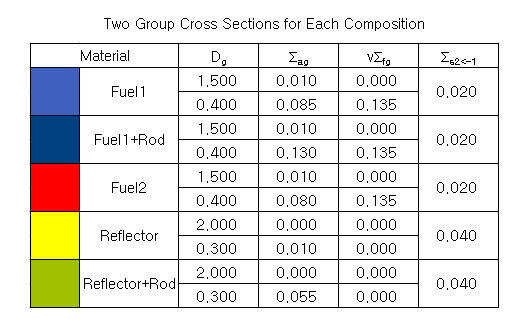
\includegraphics[width=0.5\linewidth]{xsec.png}
\end{figure}
\column{0.25\textwidth}
Image from [12]
\end{columns}
\end{frame}

%------------------------------------------------

\begin{frame}[fragile] % Need to use the fragile option when verbatim is used in the slide
\frametitle{ADPRES Input}
\begin{columns}[c] % The "c" option specifies centered vertical alignment while the "t" option is used for top vertical alignment

\column{0.70\textwidth} % Left column and width
\begin{block}{\%GEOM cards}
\begin{Verbatim}[fontsize=\tiny]
  %GEOM
  9 9 19         !nx, ny, nz
  10.0 8*20.0    !x-direction assembly size in cm
  1  8*2         !x-direction assembly divided into 2 (10 cm each)
  8*20.0 10.0    !y-direction assembly size in cm
  8*2  1         !y-direction assembly divided into 2 (10 cm each)
  19*20.0        !z-direction assembly  in cm
  19*1           !z-direction nodal is not divided
  4              !np number of planar type
  1  13*2  4*3  4     !planar assignment (from bottom to top)
  ! Planar_type_1 (Bottom Reflector)
  ....
  ....
  ! Planar_type_3 (Fuel+Partial Control Rods)
    3  2  2  2  3  2  2  1  4
    2  2  2  2  2  2  2  1  4
    2  2  3  2  2  2  1  1  4
    2  2  2  2  2  2  1  4  4
    3  2  2  2  3  1  1  4  0
    2  2  2  2  1  1  4  4  0
    2  2  1  1  1  4  4  0  0
    1  1  1  4  4  4  0  0  0
    4  4  4  4  0  0  0  0  0
  ...
  ! Boundary conditions (east), (west), (north), (south), (bottom), (top)
  1 2 2 1 1 1
\end{Verbatim}
\end{block}

\column{.3\textwidth} % Right column and width
\begin{figure}
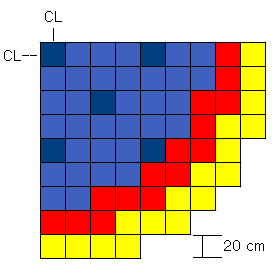
\includegraphics[width=0.7\linewidth]{iaea1.png}
\end{figure}
\begin{figure}
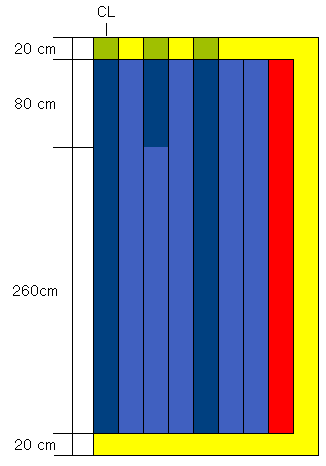
\includegraphics[width=0.7\linewidth]{iaea2.png}
\end{figure}
Image from [12]
\end{columns}
\end{frame}

%------------------------------------------------

\begin{frame}[fragile] % Need to use the fragile option when verbatim is used in the slide
\frametitle{ADPRES Input}
Point of Origin for Geometry Modelling in ADPRES
\begin{columns}[c] % The "c" option specifies centered vertical alignment while the "t" option is used for top vertical alignment

\column{0.5\textwidth} % Left column and width
\begin{figure}
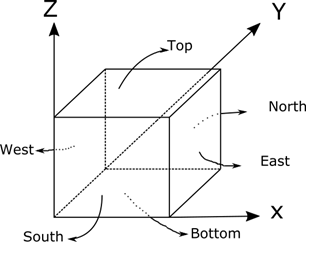
\includegraphics[width=1.0\linewidth]{geom_1.png}
\end{figure}

\column{0.5\textwidth} % Right column and width
\begin{figure}
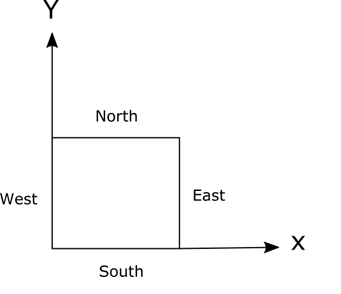
\includegraphics[width=1.0\linewidth]{geom_2.png}
\end{figure}

\end{columns}
\end{frame}

%------------------------------------------------

\begin{frame}[fragile] % Need to use the fragile option when verbatim is used in the slide
\frametitle{ADPRES Output}
\begin{block}{Output}
\begin{Verbatim}[fontsize=\tiny]
  ==============================================================================
                           CALCULATION RESULTS
  ==============================================================================

  Itr     k-eff     Fis.Src Error   Inner Error
 ----------------------------------------------------
    1     0.981424    5.47871E-01    8.55259E+03
    2     1.001319    2.41976E-01    8.56379E+00
    3     1.009804    1.67297E-01    6.27992E-01
    4     1.013500    1.33833E-01    1.44559E-01
     ...FISSION SOURCE EXTRAPOLATED...
    5     1.026980    2.65156E+00    1.31348E-01
    6     1.024050    2.69425E-01    1.90647E+00
    7     1.024688    9.31087E-02    4.43462E+01
    8     1.024358    3.99972E-02    1.10592E+00
    9     1.024191    3.47063E-02    1.96477E-01
     ...FISSION SOURCE EXTRAPOLATED...
   10     1.023838    1.12907E+00    5.87407E-02
   11     1.024188    1.12316E-01    9.62168E-01
   12     1.025744    1.03113E-01    4.24920E-01
   13     1.026299    8.09335E-02    1.86532E-01

    ...
    ...
    128     1.029082    9.48481E-06    2.04727E-05
    129     1.029082    7.46358E-06    9.66768E-06

    MULTIPLICATION EFFECTIVE (K-EFF) =  1.029082
\end{Verbatim}
\end{block}
\end{frame}

%------------------------------------------------

\begin{frame}[fragile] % Need to use the fragile option when verbatim is used in the slide
\frametitle{ADPRES Output}
\begin{block}{Output}
\begin{Verbatim}[fontsize=\tiny]
       Radial Power Distribution
     ==============================
             1       2       3       4       5       6       7       8       9
       9   0.727   1.276   1.417   1.190   0.610   0.953   0.961   0.780
       8   1.276   1.392   1.426   1.287   1.069   1.055   0.977   0.760
       7   1.417   1.426   1.364   1.308   1.179   1.089   1.001   0.715
       6   1.190   1.287   1.308   1.176   0.971   0.924   0.869
       5   0.610   1.069   1.179   0.971   0.477   0.701   0.614
       4   0.953   1.055   1.089   0.924   0.701   0.601
       3   0.961   0.977   1.001   0.869   0.614
       2   0.780   0.760   0.715
       1

     MAX POS.       Maximum Value
    (  7,  2)          1.426
\end{Verbatim}
\end{block}
\end{frame}

%------------------------------------------------

\begin{frame}[fragile] % Need to use the fragile option when verbatim is used in the slide
\frametitle{ADPRES Output}
\begin{block}{Output}
\begin{Verbatim}[fontsize=\tiny]
  Axial Power Density Distribution
====================================

  Plane Number        Power      Height
 -----------------------------------------
     19  (TOP)        0.000      380.00
     18               0.195      360.00
     17               0.353      340.00
     16               0.538      320.00
     15               0.743      300.00
     14               0.975      280.00
     13               1.182      260.00
     12               1.349      240.00
     11               1.470      220.00
     10               1.539      200.00
      9               1.554      180.00
      8               1.514      160.00
      7               1.420      140.00
      6               1.276      120.00
      5               1.087      100.00
      4               0.858       80.00
      3               0.599       60.00
      2               0.348       40.00
      1  (BOTTOM)     0.000       20.00

MAX POS.       Maximum Value
 (  9)             1.554
\end{Verbatim}
\end{block}
\end{frame}

%------------------------------------------------

\begin{frame}[fragile] % Need to use the fragile option when verbatim is used in the slide
\frametitle{UO2-MOX PWR Transient Benchmark Results}
\begin{columns}[c] % The "c" option specifies centered vertical alignment while the "t" option is used for top vertical alignment
\column{.5\textwidth} % Left column and width
\begin{figure}
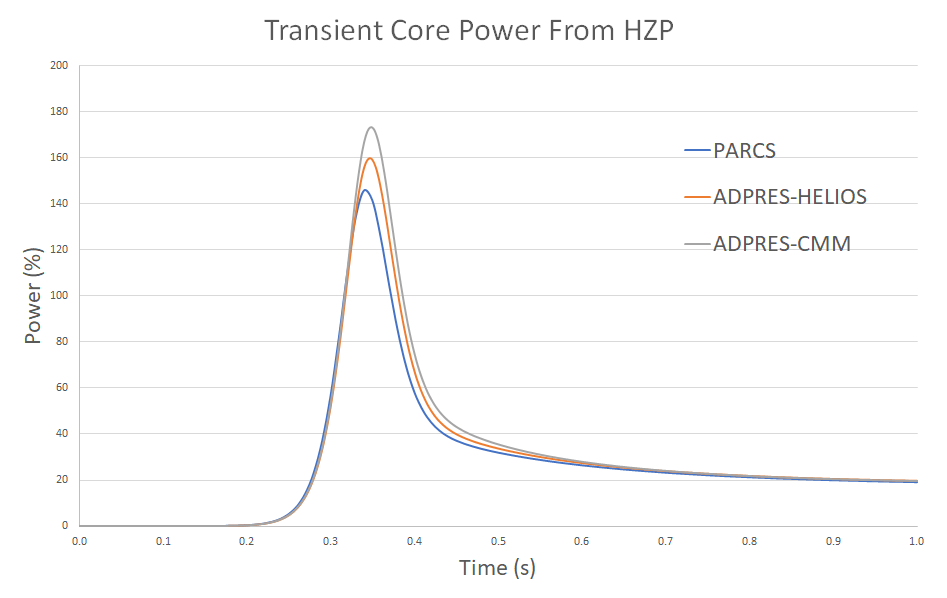
\includegraphics[width=0.9\linewidth]{power2.png}
\end{figure}
\begin{figure}
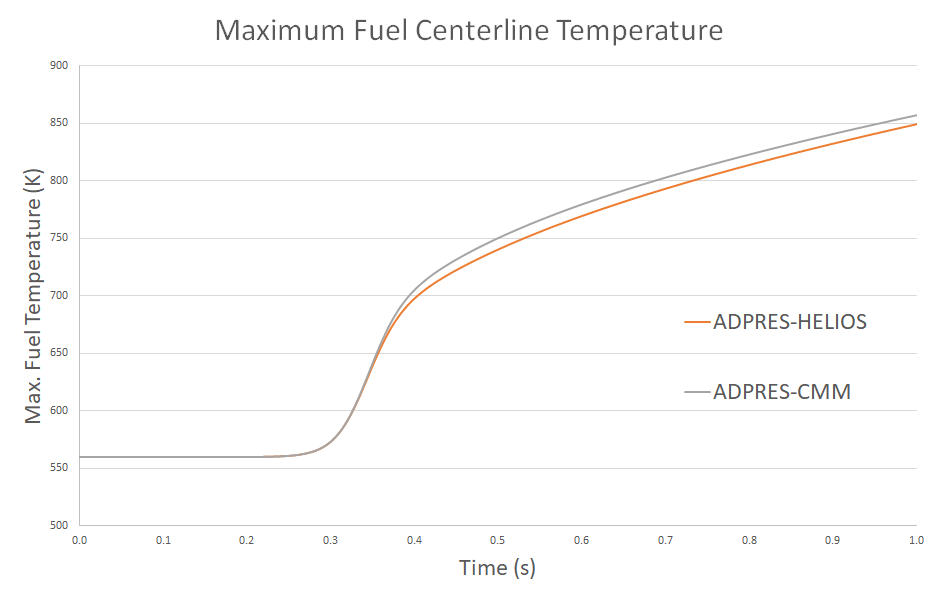
\includegraphics[width=0.9\linewidth]{ftem.png}
\end{figure}

\column{.5\textwidth} % Right column and width
\begin{figure}
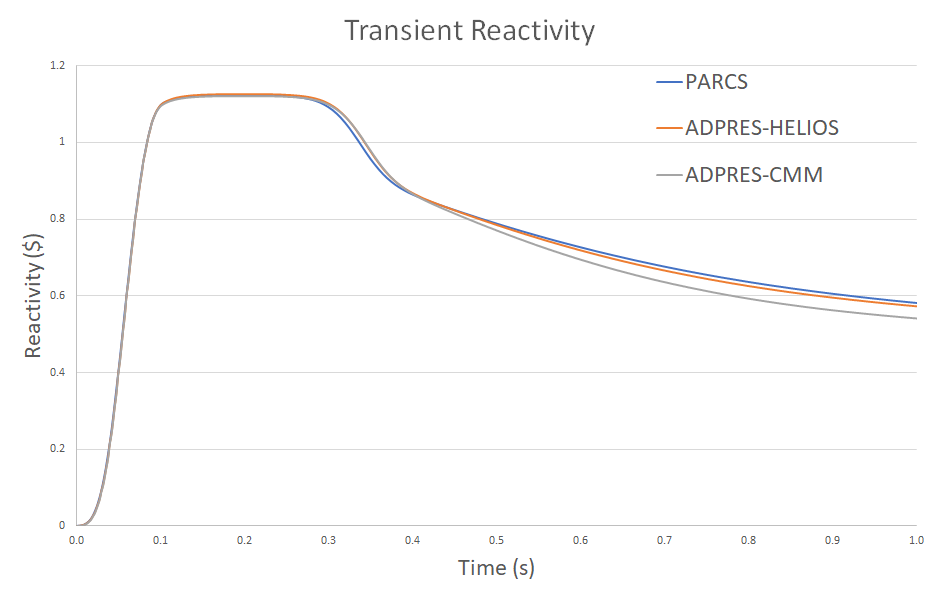
\includegraphics[width=0.9\linewidth]{reactivity.png}
\end{figure}
\begin{figure}
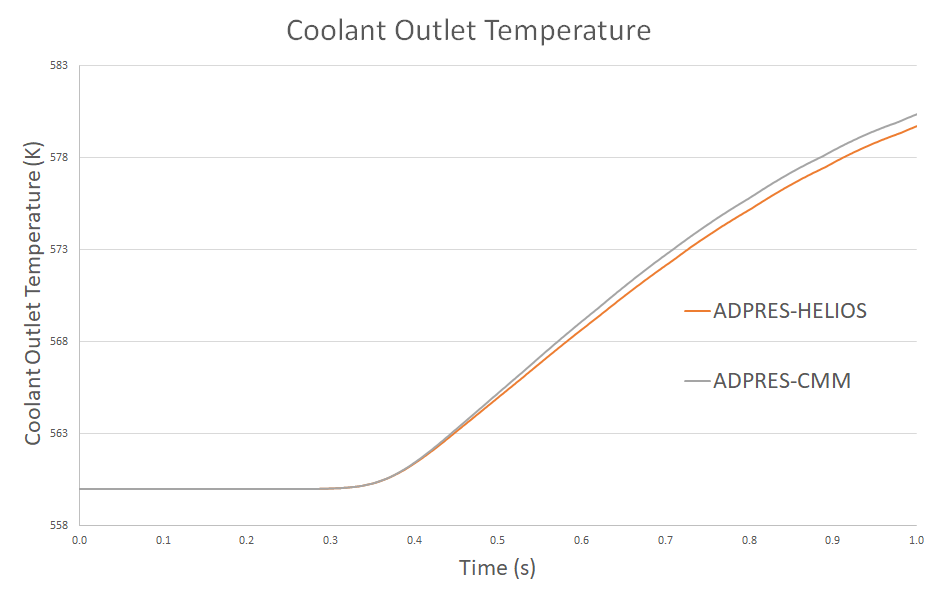
\includegraphics[width=0.9\linewidth]{mtem.png}
\end{figure}

\end{columns}

\end{frame}

%------------------------------------------------
\section{References}
%------------------------------------------------

\begin{frame}
\frametitle{References}
\begin{enumerate}
  \item Kozlowski, Thomas and Thomas J. Downar. 2007. PWR MOX/UO2 Core Transient Benchmark Final Report. Nuclear Energy Agency Organization for Economic Co-operation and Development: NEA/NSC/DOC(2006)20.
  \item McSAFE Online Training Course, 2020
  \item Finnemann, H., Bennewitz F. and Wagner M. R., 1977, Interface current techniques for multidimensional reactor calculations, Atomkernenergie, Vol. 30, pp. 123-128.
  \item Lawrence, R.D., 1986, Progress in nodal methods for the solution og the neutron diffusion and transport equations, Progress in Nuclear Energy, Vol. 17, No.3, pp. 271-301.
  \item Okumura, K., 1998, MOSRA-Light : High speed three-dimensional nodal diffusion code for vector computers, JAEA-Research 98-025. (in Japanese)
  \item K.S. Smith, Nodal Method Storage Reduction by Nonlinear Iteration, Transactions of American Nuclear Society, 44 (1984), p. 265
\end{enumerate}
\end{frame}

\begin{frame}
\frametitle{References}
\begin{enumerate}
  \setcounter{enumi}{6}
  \item Downar, T., Lee, D., Xu, Y., Kozlowski, T., Staudenmier, J., 2004. PARCS v2.6 U.S NRC Core Neutronics Simulator, Theory Manual. Draft.
  \item Turinsky, P.J., Al-Chalabi, R.M.K., Engrand, P., Sarsour, H.N., Faure, F.X., and Guo, W. (1994). NESTLE: Few-group neutron diffusion equation solver utilizing the nodal expansion method for eigenvalue, adjoint, fixed-source steady-state and transient problems (EGG-NRE--11406). United States
  \item Liem, P.H. et al., 2016. Status on development and verification of reactivity-initiated accident analysis code for PWR (NODAL3). J. Nucl. Sci. Technol. 6 (1), 1–13.
  \item Zimin, V.G. and Ninokata, H. 2003. Non-linear Iteration Procedure Based on Legendre Polynomials. Trans. Am. Nucl. Soc., 76, 162 (1997).
\end{enumerate}
\end{frame}

\begin{frame}
\frametitle{References}
\begin{enumerate}
  \setcounter{enumi}{10}
  \item Zimin, V.G. and Ninokata, H. Nodal neutron kinetics model based on nonlinear iteration procedure for LWR analysis. Ann. Nucl. Energy, 25: 507–528.
  \item Purdue Advanced Reactor Simulator (PARCS), 2002, https://engineering.purdue.edu/PARCS/Code/TestSuite /CalculationMode/StandAloneMode/Eigenvalue/IAEA3DPWR
  \item Hall, S.K., Eaton, M.D., \& Knight, M.P. (2013). The implementation of a simplified spherical harmonics semi-analytic nodal method in PANTHER. Annals of Nuclear Energy (Oxford), 280-293. doi:101016/janucene201302015
\end{enumerate}
\end{frame}

%------------------------------------------------

\begin{frame}
\Huge{\centerline{The End}}
\end{frame}

%----------------------------------------------------------------------------------------

\end{document}
